\documentclass[uplatex,12pt]{jsbook}

\RequirePackage{titlesec}
\usepackage{titlesec}
\usepackage{amsmath,amssymb}
\usepackage{euler}
\usepackage{tcolorbox}
\usepackage{picture}
\usepackage{color}
\usepackage{overpic}
%%%%%%%%%%%%%%%%%%%%%%%%%%%
%Jotaro-MACROS
\newcommand{\strong}[1]{{\textbf{\color{violet} #1}}}

%%%%%%%%%%%%%%%%%%%%%%%%%%%

%For Gothic Japanese Font
%\renewcommand{\kanjifamilydefault}{\gtdefault}

\definecolor{white}{RGB}{255,255,255}
\definecolor{violet}{RGB}{231,26,116}
\definecolor{lightviolet}{RGB}{255,96,156}
\definecolor{teal}{RGB}{0,128,128}
\definecolor{powderblue}{RGB}{176,224,230}
\definecolor{darkslateblue}{RGB}{72,61,139}
\definecolor{darkslategray}{RGB}{47,79,79}
\definecolor{lightcyan}{RGB}{224,255,255}

% chapter                                                                                                                                                                                                                                                                                                                                                              
\titleformat{\chapter}[block]
{}{}{5pt}{
	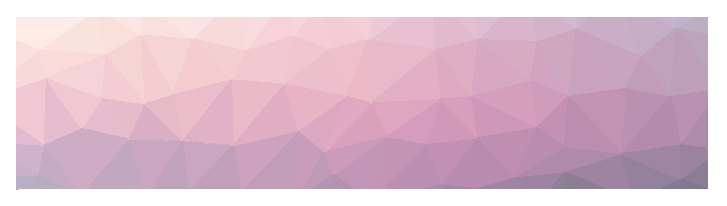
\includegraphics[width=3cm ,bb = 0 0 65 30]{chapterback.eps}\color{violet}
	\hspace{-1in}\fontsize{35pt}{40pt}\selectfont\sf\raisebox{0.5in}
}[
\color{black}\sf\Large\filleft{ CHAPTER \Huge\thechapter}
]


% section                                                                                                                                                                                                                                                                                                                                                              
\titleformat{\section}[block]
{}{}{0pt}
{
		\begin{overpic}[width=3cm ,bb = -4 3 100 90]{sectionback.eps}
			\put(53,2){\color{white}\sf\Huge\,\,\,\,\,\,\,\,\,\,\,\,\thesection}
		\end{overpic}
	\normalfont \huge \sf \color{violet}\,\,\,\,\,\,\,\,\,\,\,\,\,
}
[
\begin{picture}(100,0)
%\put(3,30){\color{teal}\line(1,0){400}}
\end{picture}
\\
\vspace{-50pt}
]

% subsection                                                                                                                                                                                                                                                                                                                                                           
\titleformat{\subsection}[block]
{}{}{0pt}
{
	\colorbox{lightviolet}{\begin{picture}(0,10)\end{picture}}
	\hspace{0pt}
	\normalfont \Large\bfseries \thesubsection
	\hspace{-4pt}
}
[
\begin{picture}(100,0)
\end{picture}
\\
\vspace{-40pt}
]

% margin                           
\setlength{\textwidth}{155truemm}
\addtolength{\evensidemargin}{0in}                                                                                                                                                                                                                                                                                                                                   
\addtolength{\textheight}{0in}
\addtolength{\marginparwidth}{0in}
\addtolength{\voffset}{-0.3in}
\setlength{\oddsidemargin}{0in}
\parindent=0zw

\pagestyle{headings}
\begin{document}
	\chapter{序章}
	\section{流れ学第1の復習}
	\subsection{流れ学第1との違い}
	流れ学第1では主に,質量・運動量・角運動量・エネルギの保存則を用いて流体の振る舞いについて論じました.流れ学第2では,NS方程式をはじめとして主に微分方程式を支配方程式として流体の運動を記述していくことになります.
	
	\subsection{流体の性質と運動方程式}
	\subsubsection{流体力学の,他の力学との相違}
	流体力学は連続体の力学の一種ですが,連続体には材料力学のように固体の場合と,流体力学の液体の場合があります.個体の場合は,一例ですと,以下に代表される\strong{フックの法則}
	\begin{equation}
		F = k\Delta x
	\end{equation}
	といった,変位に応じた力が記述されますが,流体の場合は機械力学で出てきたオイルダンパと同様に
	\begin{equation}
	F = c \frac{dx}{dt}
	\end{equation}
	速度に応じた,いわゆる\strong{粘性抵抗}が働きます.
	
	\subsubsection{ニュートンの粘性法則}
	流体中に,速度$u(y)$で動いている分子が衝突する際の運動量交換について調べてみます.基準点と,基準点から分子運動の平均行程$\lambda$だけ離れた点の,質量$m$の分子の運動量変化は
	\begin{equation}
		\Delta M = m\left(u(0)-u(\lambda)\right) \label{eq:Momentum Variation1}
	\end{equation}
	ここで$u(-\lambda)$を$-\lambda$周りにTaylor展開\footnote{$f(x+\epsilon) = f(x) + f'(x)\epsilon + f''(x)\frac{\epsilon^2}{2!}...$\\}します.
	\begin{align}
		u(-\lambda) &= u(0) -\lambda\frac{du}{dy} + o(\epsilon^2)\\
		&\approx u(0) -\lambda\frac{du}{dy} \label{eq:Taylor1}
	\end{align}
	式(\ref{eq:Momentum Variation1})に式(\ref{eq:Taylor1})を代入して
	\begin{equation}
		\Delta M = -m\lambda\frac{du}{dy}
	\end{equation}
	が成り立ちます.ここで,流体に加わるせん断応力$\tau$は,分子の数密度・運動量変化・その点での分子の平均速度に比例します.
	\begin{align}
		\tau &\propto \Delta MN\overline{u_m}\\
		&= m\lambda N\overline{u_m}\frac{du}{dy}
	\end{align}
	ここで,流体密度$\rho = mN$より,
	\begin{equation}
		\tau \propto \rho\lambda\overline{u_m}\frac{du}{dy}
	\end{equation}
	が成り立っており,分子の平均速度をエネルギー等配分の法則に基づいて計算すると,
	\begin{equation}
	\tau = \underbrace{\frac{\rho\lambda\overline{u_m}}{3}}_{\color{violet}{\mu = \rm{粘性係数}}}\frac{du}{dy}
	\end{equation}
	が成り立つことが知られています.このようなアプローチで流体中のせん断応力が速度勾配に比例するという性質,すなわち\strong{ニュートンの粘性法則}を導くことができます.また,このような性質を持つ流体は\strong{ニュートン流体}と呼ばれています.
	\chapter{NAVIER STOKES wwww}
	\section{流れ学第1の復習}
	\subsection{流れ学第1との違い}
	\subsubsection{サブサブセクション}
	ながれがくああながれがくながれがくながれがくああながれがくながれがくながれがくああながれがくながれがくながれがくああながれがくながれがくながれがくああながれがくながれがくながれがくああながれがくながれがくながれがくああながれがくながれがくながれがくああながれがくながれがくながれがくああながれがくながれがくながれがくああながれがくながれがくながれがくああながれがくながれがくながれがくああながれがくながれがくながれがくああながれがくな,な,な,ななななNavier Stokes
	\[
		\frac{D\bf V}{Dt} = -\nabla p + \nu\nabla^2\bf V + \bf F
	\]だめーwwwだめーwwwだめーwwwだめーwwwだめーwwwだめーwwwだめーwwwだめーwwwだめーwwwだめーwwwだめーwwwだめーwwwだめーwwwだめーwwwだめーwwwだめーwwwだめーwwwだめーwwwだめーwwwだめーwwwだめーwwwだめーwwwだめーwwwだめーwwwだめーwwwだめーwwwだめーwwwだめーwwwだめーwwwだめーwwwだめーwwwだめーwwwだめーwwwだめーwwwだめーwwwだめーwwwだめーwwwだめーwwwだめーwwwだめーwwwだめーwww
	\subsection{流れ学第1との違い}
	\subsubsection{サブサブセクション}
	ながれがくああながれがくながれがくながれがくああながれがくながれがくながれがくああながれがくながれがくながれがくああながれがくながれがくながれがくああながれがくながれがくながれがくああながれがくながれがくながれがくああながれがくながれがくながれがくああながれがくながれがくながれがくああなが
	ながれがくああながれがくながれがくながれがくああながれがくながれがくながれがくああながれがくながれがくながれがくああながれがくながれがくながれがくああながれがくながれがくながれがくああながれがくながれがくながれがくああながれがくながれがくながれがくああながれがくながれがくながれがくああなが
	ながれがくああながれがくながれがくながれがくああながれがくながれがくながれがくああながれがくながれがくながれがくああながれがくながれがくながれがくああながれがくながれがくながれがくああながれがくながれがくながれがくああながれがくながれがくながれがくああながれがくながれがくながれがくああなが
	
\end{document}